\chapter{Results}

The classifiers developed in this replication attempt were constructed and evaluated according to the parameters
and metrics described in Section~\ref{sec:modelflex}. Figure~\ref{fig:modelPerformance} shows the sensitivity 
and specificity of each tested model alongside the performance of the originally published model (on AAC feature set), 
with 10\% of models most closely matching performance to the reference highlighted.

Tables~\ref{tab:prob_7class} contains the complete performance of the probability-based models
being evaluated using each the performance metrics in~\cite{mishra_prediction_2014} for the 7-class settings. 
Among all the models, 8 reported the closest performance with the distance values between $0.07$ and $0.13$
from the reference. Tables~\ref{tab:prob_8class} shows the performance of the probability-based models through the 
8-class settings with the closest performance values between $0.08$ and $0.10$ for 8 models. 
In both of those settings mentioned above, the models were all aggregated using balanced averaging technique and 
the performance results were calculated using micro averaging technique. 
Table~\ref{tab:scikit_pred} shows the same for the Scikit-Learn Prediction models. Through this setting, 
all the models reported the distance values above $0.32$ from the reference.

Table~\ref{tab:dpcPhcAaindexPssm},~\ref{tab:aacDpcPhcAaindexPssm},~\ref{tab:dpcPhcAaindexPssmAaindexPhc},
~\ref{tab:aacDpcAaindexPssmHybrid3},~\ref{tab:aacAaindexPhcPssmHybrid3}
contain the performance metrics values from running the closest models settings ($10\%$ being selected from 
the AAC experiment) when applied to all the other 18 features. 
Table~\ref{tab:dpcPhcAaindexPssm} shows the results from running the $10\%$ (16) best models on DPC, PHC, 
AAindex and PSSM feature sets. They all reported the distance values between $0.06$ and $0.13$ from the reference. 
The models being built on DPC feature set seems to perform slightly better in 7-class settings while for the 
other 3 feature sets performance is quite close through both 7- and 8-class settings.

Tables~\ref{tab:aacDpcPhcAaindexPssm},~\ref{tab:dpcPhcAaindexPssmAaindexPhc} shows the results from running 
the $10\%$ (16) best models on hybrid sets when 2 feature sets are combined (8). All the models reported 
the distance values between $0.06$ and $0.13$ from their correspondent reference point in~\cite{mishra_prediction_2014}. 
The models being built on DPC+AAC, DPC+PSSM and DPC+AAINDEX hybrid feature sets seems to perform slightly better 
in 7-class settings while the results from all the other 5 feature sets shows a close performance through 
both 7- and 8-class settings.

Tables~\ref{tab:aacDpcAaindexPssmHybrid3},~\ref{tab:aacAaindexPhcPssmHybrid3} shows the results from running 
the $10\%$ (16) best models on hybrid sets when 3 feature sets are combined (6). All the models reported 
the distance values between $0.06$ and $0.11$ from their correspondent reference. The hybrid AAC+DPC+AAINDEX 
model seems to perform slightly better in 7-class settings while all the models using all the other 5 hybrid 
feature sets shows a close performance through both 7- and 8-class settings.

Figure~\ref{fig:MccAllModels} compares the MCC values resulted 
from running the closest models settings on all the other 18 features. Finally, Table~\ref{tab:pssmAaindex} 
shows the results from running the best-performing models on the main and independent datasets for the 
hybrid model that included the biochemical composition and the PSSM profile. All the models (16) reported 
the distance values between $0.07$ and $0.09$ from the reference. According to~\cite{mishra_prediction_2014},
compared to the other feature sets, this hybrid features set produces the best results for the 
membrane protein classification with the highest MCC values. 
Figure~\ref{fig:MccAllModels} shows that the MCC value being calculated for this 
feature set is higher than the other models being built using other 18 feature sets.

\section{Models Differences}
The remainder of this section will explore the differences in model performance based on the defined axes of
flexibility enumerated in Section~\ref{sec:experimentaldesign}.

\begin{figure}[ht]
    \centering
    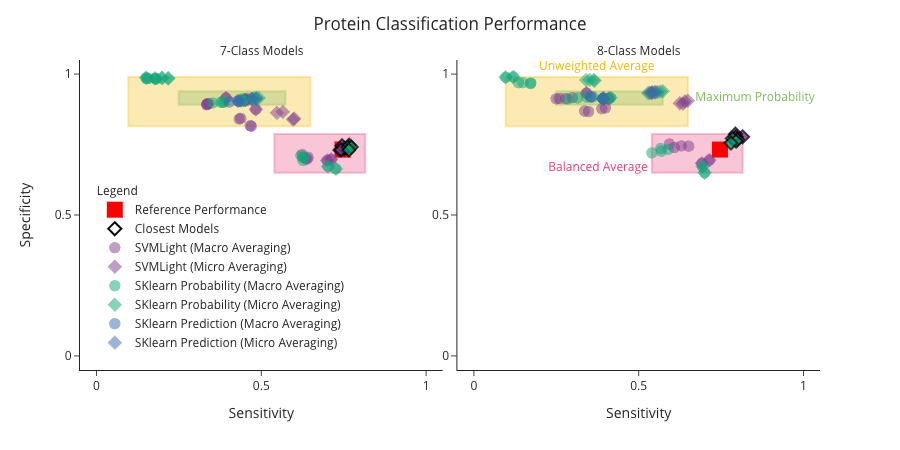
\includegraphics[width=0.90\textwidth]{figures/14ModelPerformance.png}
    \caption{Sensitivity and Specificity of each tested model. Each panel contains models 
    trained with a fixed number of categories (7: left; 8: right), and shows the published 
    reference performance in red. The closest 10\% of models to this reference have been 
    outlined in black. The symbol colour and shape refer to the classifier type and aggregation 
    strategy, respectively. Each shaded region illustrates the bounds of performance for a given 
    binary classifier aggregation strategy.}
    \label{fig:modelPerformance}
\end{figure}

\paragraph{Number of Classes}
While the 7-class models appear to be slightly closer to the reference, there was no significant difference between
the number of classes and the distance from reference ($p > 0.1$). Models trained with 8 classes tended to achieve
higher sensitivity and specificity values. It seems that the addition of the background class has improve the 
performance.

\paragraph{Dataset Sampling}
The dataset composition had no significant impact on the closeness of the model to the reference ($p > 0.1$ for all
comparisons). However, none of the closest 10\% of models were trained using the downsampled dataset.

\paragraph{SVM Hyperparameters}
All uniformly parameterized models converged to same set of hyperparameters within the number of classes. For the 
models with 7-classes of proteins, the ones with the closest performance used Gamma and Cost 
values of $0.02$ and $4.5$ while for the models with 8-classes of proteins, the closest results were achieved using 
the values of $0.01$ and $4$ for Gamma and Cost respectively. There was no significant difference between these 
sets of parameters.

\paragraph{Hypterparamter Heterogeneity}
Similarly to the case of uniform parameters, models converged on Gamma values between $0.02$ and $0.04$ for all classes
and models, and Cost values between $4$ and $5$, with no statistically significant difference between models or classes.

\paragraph{Aggregation Technique}
Models using the micro performance-aggregation technique (i.e. evaluating individual binary classifiers prior to
aggregation into a multi-class classifier) obtained closer results to the reference than those using the macro
technique ($p < 1\times 10^{-4}$). All of the closest models used micro-aggregation.

\paragraph{Prediction Method}
The balanced averaging prediction method produced significantly closer results to the reference than both the
unweighted average and maximum probability methods ($p < 1\times 10^{-5}$ for both). The maximum probability method
also produced significantly closer results than the unweighted average method ($p < 0.001$).

\paragraph{Tool}
The SVMLight classifiers produced closer results to the reference than both Scikit-Learn Probability and Prediction models
($p < 0.05$ for both). While the Scikit-Learn Prediction model architecture did not appear in the set of closest models,
there was no statistically significant difference between its performance and that of the Scikit-Learn Probability models.

\section{Closest Models}
% \paragraph{Closest Models}
The closest 10\% of models (16) used a variety of configurations, and each reported a distance score of less than
$0.13$ from the reference. The breakdown of configurations for these models included: micro aggregation (all), balanced
average prediction method (all), balanced (8) or shuffled (8) dataset, contained 7 (8) or 8 (8) classes in the dataset,
were trained with uniform (8) or heterogeneous (8) hyperparameters, and were developed using SVMLight (8) or the
Scikit-Learn Probability (8) model architectures. While the Scikit-Learn Prediction model and downsampled dataset configuration
are notably absent from these models, all other settings were either dominated by a single value, such as in the case
of micro aggregation and the balanced average prediction method, or the settings were equally represented. This
uniformity in representation is consistent with the direct comparisons between settings described above.

For all the other 18 feature sets (DPC, PHC, PSSM, AAINDEX and 14 hybrid feature sets) the closest 10\% of the models (16) 
each reported a distance score of less than $0.13$ from the feature's reference values. 
Figure~\ref{fig:MccAllModels} shows the MCC values resulted from running 
the closest 10\% models (16) on all the features (19). 
The hybrid dataset that included the biochemical composition (AAindex) and the PSSM profile 
outperforms others. For this hybrid feature set, the reported distance from the reference values 
for the closest models (Table~\ref{tab:pssmAaindex}) 
were between $0.09$ and $0.07$ on the main dataset and between $0.08$ and $0.02$ on the independent dataset.

%Tables
\begin{table}[ht]
    \scriptsize
    \begin{adjustwidth}{-1.0in}{40in} 
        \centering
        \begin{tabular}{|L | V |V V V V g g g V V V V | V |}
            \hline
            \multicolumn{14}{|g|}{7-class based model for AAC}\\
            \hline
            \multicolumn{1}{|l|}{\multirow{2}{*}{\footnotesize{Original Results}}}
            &
            \multicolumn{3}{g}{Accuracy} & \multicolumn{3}{g}{Sensitivity} &
            \multicolumn{3}{g}{Specificity} & \multicolumn{4}{g|}{MCC}\\
            \cline{2-14}&
            \multicolumn{3}{C}{73.74} & \multicolumn{3}{C}{74.65} &
            \multicolumn{3}{C}{73.22} & \multicolumn{4}{C|}{0.46} \\
            \hline\hline
            
            \multicolumn{14}{|g|} {SVM Light}\\
            \hline\hline
            
            \cline{1-12}\multicolumn{1}{|g}{}&
            
            \multicolumn{1}{|g|}{\footnotesize{Dist}}&
            \multicolumn{4}{g} {\footnotesize{Gamma-Cost different for each class}}&
            \multicolumn{3}{g}{}&
            \multicolumn{4}{g|} {\footnotesize{same Gamma-Cost for all classes}}&
            \multicolumn{1}{g|}{\footnotesize{Dist}}\\
            
            \cline{3-6}\cline{10-13}\multicolumn{1}{|g}{}&
            \multicolumn{1}{|g|}{\footnotesize{ance}}&
            \multicolumn{1}{g}{acc}&\multicolumn{1}{g}{sens}&
            \multicolumn{1}{g}{spec}&\multicolumn{1}{g}{mcc}&
            \multicolumn{3}{g}{}&
            \multicolumn{1}{g}{acc}&\multicolumn{1}{g}{sens}&
            \multicolumn{1}{g}{spec}&\multicolumn{1}{g|}{mcc}&\multicolumn{1}{g|}{\footnotesize{ance}}\\
    
            \hline
            % \multicolumn{1}{|l|}{\multirow{6}{*}{\footnotesize{unweighted average}}}
            & 0.25 & 82.28 & 56.53 & 86.58 & 0.37 &    b&&b                & 80.73 & 60.00 & 84.18 & 0.37 & 0.21 \\
            & 0.43 & 84.07 & 39.28 & 91.55 & 0.32 &    d&\footnotesize{Micro}&d   & 81.90 & 48.33 & 87.5 & 0.32 & 0.33 \\
            \multicolumn{1}{|c|}{\multirow{1}{*}{\footnotesize{unweighted}}}
            & 0.26 & 81.74 & 54.74 & 86.24 & 0.36 &    s&&s                & 80.42 & 59.61 & 83.88 & 0.36 & 0.21 \\
            
            \cline{2-5}\cline{7-9}\cline{11-14}
            
            \multicolumn{1}{|c|}{\multirow{1}{*}{\footnotesize{average}}}
            & 0.37 & 82.28 & 43.76 & 84.31 & 0.31 &    b&&b                & 80.73 & 46.64 & 81.69 & 0.30 & 0.33 \\
            & 0.43 & 84.08 & 39.28 & 91.54 & 0.32 &    d&\footnotesize{Macro}&d   & 81.90 & 48.33 & 87.49 & 0.33 & 0.33 \\
            & 0.38 & 81.73 & 43.27 & 84.06 & 0.28 &    s&&s                & 80.42 & 46.96 & 81.49 & 0.29 & 0.33 \\
            
            \hline
            % \multicolumn{1}{|l|}{\multirow{6}{*}{\footnotesize{balanced average}}}
            &\mrkm{0.09}{73.84}{75.25}{73.60}{0.36} &    b&&b                & \mrkm{74.10}{75.12}{73.93}{0.36}{0.09} \\
            & 0.18 & 69.45 & 70.00 & 69.36 & 0.28 &     d&\footnotesize{Micro}&d   & 69.96 & 71.19 & 69.76 & 0.29 & 0.16 \\
            \multicolumn{1}{|c|}{\multirow{1}{*}{\footnotesize{balanced}}}
            &\mrkm{0.11}{72.06}{76.15}{71.39}{0.34} &    s&&s                &\mrkm{72.91}{75.38}{72.50}{0.35}{0.13} \\
            
            \cline{2-5}\cline{7-9}\cline{11-14}
            \multicolumn{1}{|c|}{\multirow{1}{*}{\footnotesize{average}}}
            & 0.20 & 73.84 & 64.18 & 70.45 & 0.28 &    b&&b                & 74.10 & 63.42 & 70.70 & 0.28 &  0.21 \\
            & 0.18 & 69.45 & 70.00 & 69.36 & 0.28 &     d&\footnotesize{Macro}&d   & 69.96 & 71.19 & 69.76 & 0.30 & 0.16 \\
            & 0.20 & 72.06 & 66.89 & 68.16 & 0.27 &     s&&s                & 72.91 & 64.46 & 69.24 & 0.26 & 0.21 \\
            
            \hline
            % \multicolumn{1}{|l|}{\multirow{6}{*}{\footnotesize{maximum probability}}}
            & 0.35 & 84.87 & 47.05 & 91.17 & 0.38 &    b&&b                & 84.54 & 45.89 & 90.98 & 0.36 & 0.36 \\
            & 0.37 & 84.35 & 45.24 & 90.87 & 0.36 &    d&\footnotesize{Micro}&d   & 83.87 & 43.57 & 90.59 & 0.34 & 0.38 \\
            \multicolumn{1}{|c|}{\multirow{1}{*}{\footnotesize{maximum}}}
            & 0.37 & 84.32 & 45.12 & 90.85 & 0.35 &    s&&s                & 84.21 & 44.74 & 90.79 & 0.35 & 0.37 \\
            
            \cline{2-5}\cline{7-9}\cline{11-14}

            \multicolumn{1}{|c|}{\multirow{1}{*}{\footnotesize{probability}}}
            & 0.48 & 84.87 & 34.05 & 89.58 & 0.28 &    b&&b                & 84.54 & 33.59 & 89.48 & 0.27 & 0.49 \\
            & 0.37 & 84.35 & 45.23 & 90.87 & 0.34 &    d&\footnotesize{Macro}&d   & 83.87 & 43.57 & 90.59 & 0.33 & 0.39 \\
            & 0.48 & 84.32 & 33.52 & 89.14 & 0.27 &    s&&s                & 84.21 & 33.47 & 89.15 & 0.27 & 0.48 \\
            
            \hline\hline
            
            \multicolumn{14}{|g|} {Scikit Learn}\\
            \hline\hline
    
            % \multicolumn{1}{|l|}{\multirow{6}{*}{\footnotesize{unweighted average}}}
            & 0.61 & 87.51 & 21.47 & 98.44 & 0.33 &    b&&b                 & 87.45 & 19.39 & 98.69 & 0.32 & 0.63 \\
            & 0.65 & 87.03 & 17.43 & 98.60 & 0.29 &    d&\footnotesize{Micro}&d   & 86.68 & 15.28 & 98.56 & 0.27 & 0.68 \\
            \multicolumn{1}{|c|}{\multirow{1}{*}{\footnotesize{unweighted}}}
            & 0.61 & 87.49 & 21.66 & 98.41 & 0.34 &    s&&s                & 87.55 & 20.878 & 98.63 & 0.34 & 0.62 \\
            
            \cline{2-5}\cline{7-9}\cline{11-14}

            \multicolumn{1}{|c|}{\multirow{1}{*}{\footnotesize{average}}}
            & 0.66 & 87.49 & 18.29 & 98.20 & 0.24 &    b&&b                 & 87.44 & 14.87 & 98.46 & 0.20 & 0.71 \\
            & 0.67 & 87.03 & 17.46 & 98.61 & 0.24 &    d&\footnotesize{Macro}&d   & 86.68 & 15.32 & 98.56 & 0.22 & 0.70 \\
            & 0.67 & 87.47 & 17.52 & 98.18 & 0.23 &    s&&s                & 87.53 & 16.32 & 98.40 & 0.21 & 0.69 \\
            
            \hline
            % \multicolumn{1}{|l|}{\multirow{6}{*}{\footnotesize{balanced average}}}
            & \mrkm{0.07}{75.33}{76.42}{75.13}{0.38} &    b&&b                 & \mrkm{75.33}{76.41}{75.15}{0.38}{0.07} \\
            & 0.20 & 68.09 & 70.95 & 67.62 & 0.27 &    d&\footnotesize{Micro}&d   & 67.31 & 70.47 & 66.78 & 0.26 & 0.21 \\
            \multicolumn{1}{|c|}{\multirow{1}{*}{\footnotesize{balanced}}}
            & \mrkm{0.07}{75.32}{76.41}{75.15}{0.38} &    s&&s                & \mrkm{73.46}{75.25}{73.16}{0.35}{0.10} \\
            
            \cline{2-5}\cline{7-9}\cline{11-14}
            
            \multicolumn{1}{|c|}{\multirow{1}{*}{\footnotesize{average}}}
            & 0.20 & 75.32 & 61.79 & 71.51 & 0.29 &    b&&b                 & 75.32 & 61.79 & 71.51 & 0.30 & 0.20 \\
            & 0.18 & 68.09 & 70.95 & 67.61 & 0.29 &    d&\footnotesize{Macro}&d   & 67.31 & 70.47 & 66.78 & 0.27 & 0.20 \\
            & 0.20 & 75.32 & 61.79 & 71.22 & 0.29 &    s&&s                & 73.46 & 61.48 & 69.51 & 0.25 & 0.24 \\
            
            \hline
            % \multicolumn{1}{|l|}{\multirow{6}{*}{\footnotesize{maximum probability}}}
            & 0.34 & 85.38 & 48.84 & 91.47 & 0.40 &    b&&b          & 85.20 & 48.20 & 91.36 & 0.39 & 0.34 \\
            & 0.37 & 84.21 & 44.76 & 90.79 & 0.35 &    d&\footnotesize{Micro}&d   & 84.14 & 44.52 & 90.75 & 0.35 & 0.37 \\
            \multicolumn{1}{|c|}{\multirow{1}{*}{\footnotesize{maximum}}}
            & 0.34 & 85.12 & 47.95 & 91.32 & 0.39 &    s&&s                & 85.12 & 47.94 & 91.32 & 0.39 & 0.34 \\
            
            \cline{2-5}\cline{7-9}\cline{11-14}
            \multicolumn{1}{|c|}{\multirow{1}{*}{\footnotesize{probability}}}
            & 0.43 & 85.38 & 38.43 & 89.98 & 0.32 &    b&&b                 & 85.20 & 37.61 & 89.90 & 0.31 & 0.44 \\
            & 0.38 & 84.21 & 44.76 & 90.79 & 0.32 &    d&\footnotesize{Macro}&d   & 84.14 & 44.52 & 90.75 & 0.33 & 0.38 \\
            & 0.44 & 85.12 & 38.33 & 89.94 & 0.31 &    s&&s                & 85.12 & 36.43 & 89.85 & 0.30 & 0.46 \\
            \hline\hline
            
            \multicolumn{14}{|c|} {\footnotesize{
                B, D and S are balanced, down-sampled and shuffled instances of the main dataset.
            }}\\
            \multicolumn{14}{|c|} {\footnotesize{
                Acc: Accuracy, Sens: Sensitivity, Spec: Specificity, Mcc: Matthews correlation coefficient
            }}\\
    
            \hline
            
           
    
        \end{tabular}
        \captionsetup{font=footnotesize,width=18cm, justification=centering}
        \caption{The average sensitivity, specificity, accuracy, and MCC  for 7 class-based models.}
        \label{tab:prob_7class}
    \end{adjustwidth}    
\end{table}
    
\begin{table}[ht]
    \scriptsize
    \begin{adjustwidth}{-1.25in}{40in}
        \centering
        \begin{tabular}{|L | V |V V V V g g g V V V V | V |}
            \hline
            \multicolumn{14}{|g|}{8-class based model for AAC}\\
            \hline
            \multicolumn{1}{|l|}{\multirow{2}{*}{\footnotesize{Original Results}}}
            &
            \multicolumn{3}{g}{Accuracy} & \multicolumn{3}{g}{Sensitivity} &
            \multicolumn{3}{g}{Specificity} & \multicolumn{4}{g|}{MCC}\\
            \cline{2-14}&
            \multicolumn{3}{C}{73.74} & \multicolumn{3}{C}{74.65} &
            \multicolumn{3}{C}{73.22} & \multicolumn{4}{C|}{0.46} \\
            \hline\hline
            
            \multicolumn{14}{|g|} {SVM Light}\\
            \hline\hline
            
            \cline{1-12}\multicolumn{1}{|g}{}&
            
            \multicolumn{1}{|g|}{\footnotesize{Dist}}&
            \multicolumn{4}{g} {Gamma-Cost different for each class}&
            \multicolumn{3}{g}{}&
            \multicolumn{4}{g|} {same Gamma-Cost for all classes}&
            \multicolumn{1}{g|}{\footnotesize{Dist}}\\
            
            \cline{3-6}\cline{10-13}\multicolumn{1}{|g}{}&
            \multicolumn{1}{|g|}{\footnotesize{ance}}&
            \multicolumn{1}{g}{acc}&\multicolumn{1}{g}{sens}&
            \multicolumn{1}{g}{spec}&\multicolumn{1}{g}{mcc}&
            \multicolumn{3}{g}{}&
            \multicolumn{1}{g}{acc}&\multicolumn{1}{g}{sens}&
            \multicolumn{1}{g}{spec}&\multicolumn{1}{g|}{mcc}&\multicolumn{1}{g|}{\footnotesize{ance}}\\
    
            \hline
    
            % \multicolumn{1}{|l|}{\multirow{6}{*}{\footnotesize{unweighted average}}}
            
            & 0.24 & 87.33 & 64.92 & 90.53 & {0.49} &    b&&b               & 86.22 & 63.40 & 89.48 & 0.46 & 0.23 \\
            & 0.49 & 85.86 & 34.16 & 93.24 & 0.30 &    d&\footnotesize{Micro}&d   & 85.02 & 40.83 & 91.34 & 0.32 & 0.42 \\
            \multicolumn{1}{|c|}{\multirow{1}{*}{\footnotesize{unweighted}}}
            & 0.24 & 87.02 & 63.98 & 90.31 & 0.48 &    s&&s                & 86.24 & 62.46 & 89.63 & 0.46 & 0.23 \\
            
            \cline{2-5}\cline{7-9}\cline{11-14}
            
            \multicolumn{1}{|c|}{\multirow{1}{*}{\footnotesize{average}}}
            & 0.43 & 87.33 & 39.91 & 88.02 & 0.30 &    b&&b               & 86.22 & 34.78 & 86.71 & 0.25 & 0.48 \\
            & 0.49 & 85.85 & 34.16 & 93.24 & 0.28 &    d&\footnotesize{Macro}&d   & 85.02 & 40.83 & 91.34 & 0.30 & 0.42 \\
            & 0.44 & 87.02 & 38.81 & 87.71 & 0.28 &    s&&s                & 86.24 & 33.57 & 86.89 & 0.23 & 0.50 \\
            
            \hline
            % \multicolumn{1}{|l|}{\multirow{6}{*}{\footnotesize{balanced average}}}
    
            & \mrkm{0.10}{79.98}{79.78}{80.01}{0.44} &    b&&b               & \mrkm{79.74}{77.97}{80.00}{0.43}{0.10} \\
            & 0.19 & 68.93 & 71.87 & 68.51 & 0.27 &     d&\footnotesize{Micro}&d   & 68.07 & 69.79 & 67.82 & 0.25 & 0.22 \\
            \multicolumn{1}{|c|}{\multirow{1}{*}{\footnotesize{balanced}}}
            & \mrkm{0.09}{77.71}{79.93}{77.40}{0.41} &     s&&s                & \mrkm{78.31}{78.33}{78.31}{0.41}{0.09} \\
            
            \cline{2-5}\cline{7-9}\cline{11-14}
    
            \multicolumn{1}{|c|}{\multirow{1}{*}{\footnotesize{average}}}
            & 0.21 & 79.59 & 57.34 & 76.24 & 0.28 &    b&&b               & 79.59 & 57.34 & 76.24 & 0.28 & 0.25 \\
            & 0.19 & 68.93 & 71.87 & 68.51 & 0.27 &     d&\footnotesize{Macro}&d   & 68.07 & 69.79 & 67.82 & 0.25 & 0.22 \\
            & 0.21 & 77.71 & 53.55 & 74.14 & 0.27 &     s&&s                & 78.31 & 58.42 & 74.72 & 0.26. & 0.26 \\
            
            \hline
            % \multicolumn{1}{|l|}{\multirow{6}{*}{\footnotesize{maximum probability}}}
    
            & 0.31 & 88.91 & 55.65 & 93.66 & {0.49} &    b&&b               & 88.51 & 54.05 & 93.43 & 0.47 & 0.32 \\
            & 0.43 & 84.84 & 39.37 & 91.33 & 0.30 &    d&\footnotesize{Micro}&d   & 84.79 & 39.16 & 91.30 & 0.30 & 0.44 \\
            \multicolumn{1}{|c|}{\multirow{1}{*}{\footnotesize{maximum}}}
            & 0.32 & 88.44 & 53.76 & 93.39 & 0.47 &    s&&s                & 88.33 & 53.33 & 93.33 & 0.46 & 0.32 \\
            
            \cline{2-5}\cline{7-9}\cline{11-14}
    
            \multicolumn{1}{|c|}{\multirow{1}{*}{\footnotesize{probability}}}
            & 0.54 & 88.91 & 29.87 & 91.65 & 0.26 &    b&&b               & 88.51 & 25.93 & 91.35 & 0.22 & 0.58 \\
            & 0.44 & 84.84 & 39.37 & 91.34 & 0.29 &    d&\footnotesize{Macro}&d   & 84.79 & 39.16 & 91.31 & 0.28 & 0.44 \\
            & 0.57 & 88.44 & 27.85 & 91.28 & 0.23 &    s&&s                & 88.33 & 24.93 & 91.22 & 0.20 & 0.60 \\
            
            \hline
            \hline
            
            \multicolumn{14}{|g|} {Scikit Learn}\\
            \hline
            \hline
    
            % \multicolumn{1}{|l|}{\multirow{6}{*}{\footnotesize{unweighted average}}}
            
            & 0.48 & 90.22 & 36.33 & 97.84 & 0.46  &    b&&b               & 90.11 & 35.22 & 97.92 & 0.45 & 0.49 \\
            & 0.72 & 88.10 & 12.18 & 98.86 & 0.23 &    d&\footnotesize{Micro}&d   & 87.75 & 9.63 & 98.86 & 0.19 & 0.76  \\
            \multicolumn{1}{|c|}{\multirow{1}{*}{\footnotesize{unweighted}}}
            & 0.48 & 90.10 & 36.52 & 97.68 & 0.45 &    s&&s                & 89.89 & 33.28 & 97.96 & 0.43 & 0.50 \\
            
            \cline{2-5}\cline{7-9}\cline{11-14}

            \multicolumn{1}{|c|}{\multirow{1}{*}{\footnotesize{average}}}
            & 0.68 & 90.19 & 17.30 & 96.85 & 0.22 &    b&&b               & 90.10 & 15.26 & 96.98 & 0.17 & 0.71 \\
            & 0.74 & 88.10 & 12.21 & 98.86 & 0.18 &    d&\footnotesize{Macro}&d   & 87.75 & 9.71 & 8.86 & 0.13 & 0.78  \\
            & 0.68 & 90.07 & 17.17 & 96.68 & 0.20 &    s&&s                & 89.88 & 12.90 & 97.02 & 0.15 & 0.74 \\
            
            \hline
            % \multicolumn{1}{|l|}{\multirow{6}{*}{\footnotesize{balanced average}}}
    
            & \mrkm{0.08}{77.08}{80.0}{76.66}{0.40}  &     b&&b               & \mrkm{77.70}{78.18}{77.63}{0.40}{0.08} \\
            & 0.22 & 67.91 & 69.16 & 67.73 & 0.25 &     d&\footnotesize{Micro}&d   & 68.75 & 67.28 & 68.96 & 0.25 & 0.23  \\
            \multicolumn{1}{|c|}{\multirow{1}{*}{\footnotesize{balanced}}}
            & \mrkm{0.08}{76.66}{78.47}{76.40}{0.39} &     s&&s                & \mrkm{74.36}{79.41}{73.64}{0.37}{0.09} \\
            
            \cline{2-5}\cline{7-9}\cline{11-14}

            \multicolumn{1}{|c|}{\multirow{1}{*}{\footnotesize{average}}}
            & 0.24 & 77.08 & 59.13 & 73.10 & 0.27 &     b&&b               & 77.70 & 54.72 & 74.14 & 0.25 & 0.28 \\
            & 0.21 & 67.91 & 69.16 & 67.73 & 0.26 &     d&\footnotesize{Macro}&d   & 68.75 & 67.29 & 68.95 & 0.26 & 0.22  \\
            & 0.27 & 76.66 & 56.55 & 72.78 & 0.25 &     s&&s                & 74.36 & 56.27 & 0.07 & 0.22 & 0.30 \\
            
            \hline
            % \multicolumn{1}{|l|}{\multirow{6}{*}{\footnotesize{maximum probability}}}
    
            & 0.31 & 89.33 & 57.31 & 93.90 & 0.51 &     b&&b         & 88.73 & 54.92 & 93.56 & 0.48 & 0.32 \\
            & 0.42 & 85.10 & 40.41 & 91.49 & 0.31 &     d&\footnotesize{Micro}&d   & 85.31 & 41.25 & 91.60 & 0.32 & 0.41  \\
            \multicolumn{1}{|c|}{\multirow{1}{*}{\footnotesize{maximum}}}
            & 0.31 & 89.09 & 56.37 & 93.76 & 0.50 &     s&&s                & 88.15 & 52.60 & 93.22 & 0.45 & 0.33 \\
            
            \cline{2-5}\cline{7-9}\cline{11-14}

            \multicolumn{1}{|c|}{\multirow{1}{*}{\footnotesize{probability}}}
            & 0.47 & 89.32 & 36.12 & 91.94 & 0.34 &     b&&b               & 88.73 & 31.39 & 91.51 & 0.29 & 0.52 \\
            & 0.43 & 85.10 & 40.41 & 91.48 & 0.30 &     d&\footnotesize{Macro}&d   & 85.31 & 41.25 & 91.60 & 0.31 & 0.42  \\
            & 0.49 & 89.09 & 33.78 & 91.73 & 0.30 &     s&&s                & 88.15 & 28.05 & 91.14 & 0.23 & 0.56 \\
            \hline\hline
            
            \multicolumn{14}{|c|} {\footnotesize{
                B, D and S are balanced, down-sampled and shuffled instances of the main dataset.
            }}\\
            \multicolumn{14}{|c|} {\footnotesize{
                Acc: Accuracy, Sens: Sensitivity, Spec: Specificity, Mcc: Matthews correlation coefficient
            }}\\
    
            \hline
            
           
    
        \end{tabular}
        \captionsetup{font=footnotesize,width=18cm, justification=centering}
        \caption{The average sensitivity, specificity, accuracy, and MCC  for 8 class-based models.}
        \label{tab:prob_8class}
        
    \end{adjustwidth}
\end{table}
    
    
    
\input{tables/3aacprediction.tex}
\begin{table}[ht]
    \scriptsize
    \begin{adjustwidth}{-0.75in}{40in}
        \centering
        \begin{tabular}{| C | C | V |V V V V g g g V V V V | V |}
            
            \hline
            \multicolumn{15}{|g|} {PSSM + AAindex}\\
            \hline\hline
            
            \cline{1-13}
            \multicolumn{1}{|g}{\footnotesize{number of}}&
            \multicolumn{1}{|g}{\footnotesize{gamma}}&
            \multicolumn{1}{|g|}{\footnotesize{Dist}}&
            \multicolumn{4}{g} {main}&
            \multicolumn{3}{g}{}&
            \multicolumn{4}{g|} {independent}&
            \multicolumn{1}{g|}{\footnotesize{Dist}}\\
            
            \cline{4-7}\cline{11-14}
            \multicolumn{1}{|g}{\footnotesize{classes}}&
            \multicolumn{1}{|g}{\footnotesize{cost}}&
            \multicolumn{1}{|g|}{\footnotesize{ance}}&
            \multicolumn{1}{g}{acc}&\multicolumn{1}{g}{sens}&
            \multicolumn{1}{g}{spec}&\multicolumn{1}{g}{mcc}&
            \multicolumn{3}{g}{}&
            \multicolumn{1}{g}{acc}&\multicolumn{1}{g}{sens}&
            \multicolumn{1}{g}{spec}&\multicolumn{1}{g|}{mcc}&
            \multicolumn{1}{g|}{\footnotesize{ance}}\\
    
            \hline

            \multicolumn{1}{|c|}{\multirow{8}{*}{\footnotesize{7}}}
            & \multicolumn{1}{|c|}{\multirow{2}{*}{\footnotesize{different}}}
            
            &  0.07 & 77.76 & 77.57 & 77.80 & 0.42 &    b&                       &b   & 76.50 & 72.00 & 77.25 & 0.37 & 0.05 \\
            && 0.07 & 77.32 & 77.69 & 77.26 & 0.42 &    sh&\footnotesize{scikit}&sh   & 75.78 & 73.83 & 76.11 & 0.37 & 0.05 \\
            
            \cline{2-6}\cline{12-15}
            
            & \multicolumn{1}{|c|}{\multirow{2}{*}{\footnotesize{same}}}
            &  0.07 & 76.74 & 78.72 & 76.41 & 0.42 &    b&\footnotesize{learn} &b    & 75.71 & 73.34 & 76.11 & 0.37 & 0.05 \\
            && 0.07 & 76.99 & 77.95 & 76.84 & 0.42 &    sh&                    &sh   & 75.38 & 73.83 & 75.64 & 0.37 & 0.05 \\
            
            \cline{2-15}

            &\multicolumn{1}{|c|}{\multirow{2}{*}{\footnotesize{different}}}
            &  0.09 & 76.10 & 76.41 & 76.05 & 0.40 &    b&                    &b   & 74.24 & 70.67 & 74.84 & 0.34 & 0.08 \\
            && 0.08 & 77.13 & 76.03 & 77.31 & 0.41 &    sh&\footnotesize{svm}&sh   & 74.60 & 69.67 & 75.42 & 0.34 & 0.08 \\
            
            \cline{2-6}\cline{12-15}
            
            &\multicolumn{1}{|c|}{\multirow{2}{*}{\footnotesize{same}}}
            &  0.09 & 75.88 & 78.20 & 75.49 & 0.40 &    b&\footnotesize{light} &b    & 74.60 & 75.50 & 74.44 & 0.37 & 0.06 \\
            && 0.09 & 76.12 & 77.69 & 75.85 & 0.40 &    sh&                    &sh   & 74.67 & 75.33 & 74.55 & 0.37 & 0.06 \\
            
            \hline

            \multicolumn{1}{|c|}{\multirow{8}{*}{\footnotesize{8}}}
            & \multicolumn{1}{|c|}{\multirow{2}{*}{\footnotesize{different}}}
            &  0.08 & 80.89 & 80.80 & 80.90 & 0.46 &    b&                       &b   & 79.57 & 77.33 & 79.89 & 0.43 & 0.02 \\
            && 0.09 & 81.73 & 81.96 & 81.70 & 0.48 &    sh&\footnotesize{scikit}&sh   & 79.63 & 77.11 & 79.98 & 0.42 & 0.02 \\
            
            \cline{2-6}\cline{12-15}
            
            & \multicolumn{1}{|c|}{\multirow{2}{*}{\footnotesize{same}}}
            &  0.08 & 80.80 & 80.94 & 80.78 & 0.46 &    b&\footnotesize{learn} &b    & 79.85 & 77.66 & 80.16 & 0.43 & 0.02 \\
            && 0.09 & 81.58 & 81.81 & 81.54 & 0.48 &    sh&                    &sh   & 79.89 & 77.44 & 80.24 & 0.43 & 0.02 \\
       
            \cline{2-15}

            &\multicolumn{1}{|c|}{\multirow{2}{*}{\footnotesize{different}}}
            &  0.08 & 80.77 & 78.05 & 81.16 & 0.45 &    b&                    &b   & 78.94 & 71.78 & 79.97 & 0.39 & 0.02 \\
            && 0.08 & 81.42 & 78.41 & 81.85 & 0.46 &    sh&\footnotesize{svm}&sh   & 79.20 & 71.45 & 80.30 & 0.39 & 0.02 \\
            
            \cline{2-6}\cline{12-15}
            
            &\multicolumn{1}{|c|}{\multirow{2}{*}{\footnotesize{same}}}
            &  0.08 & 81.11 & 80.14 & 81.25 & 0.46 &    b&\footnotesize{light} &b    & 79.24 & 78.55 & 79.33 & 0.43 & 0.02 \\
            && 0.08 & 81.35 & 81.09 & 81.39 & 0.47 &    sh&                    &sh   & 79.51 & 77.56 & 79.79 & 0.43 & 0.02 \\
            
            \hline
            
            \multicolumn{15}{|c|} {\footnotesize{
                b and sh are balanced and shuffled instances of the main dataset.
            }}\\
            \multicolumn{15}{|c|} {\footnotesize{
                Acc: Accuracy, Sens: Sensitivity, Spec: Specificity, Mcc: Matthews correlation coefficient
            }}\\
    
            \hline
    
        \end{tabular}
        \captionsetup{font=footnotesize,width=18cm, justification=centering}
        \caption{The results from running 10\% best models on the hybrid feature set including AAindex and PSSM 
        for both main and independent datasets. This feature set outperfms the other 18 combinations.}
        \label{tab:pssmAaindex}
        
    \end{adjustwidth}
\end{table}
    
    
    
\begin{table}[ht]
    \scriptsize
    \begin{adjustwidth}{-0.95in}{40in}
        \centering
        \begin{tabular}{| C | C | V |V V V V g g g V V V V | V |}
            
            \hline
            \cline{1-13}
            \multicolumn{1}{|g}{\footnotesize{number of}}&
            \multicolumn{1}{|g}{\footnotesize{gamma}}&
            \multicolumn{1}{|g|}{\footnotesize{Dist}}&
            \multicolumn{4}{g} {dpc}&
            \multicolumn{3}{g}{}&
            \multicolumn{4}{g|} {phc}&
            \multicolumn{1}{g|}{\footnotesize{Dist}}\\
            
            \cline{4-7}\cline{11-14}
            \multicolumn{1}{|g}{\footnotesize{classes}}&
            \multicolumn{1}{|g}{\footnotesize{cost}}&
            \multicolumn{1}{|g|}{\footnotesize{ance}}&
            \multicolumn{1}{g}{acc}&\multicolumn{1}{g}{sens}&
            \multicolumn{1}{g}{spec}&\multicolumn{1}{g}{mcc}&
            \multicolumn{3}{g}{}&
            \multicolumn{1}{g}{acc}&\multicolumn{1}{g}{sens}&
            \multicolumn{1}{g}{spec}&\multicolumn{1}{g|}{mcc}&
            \multicolumn{1}{g|}{\footnotesize{ance}}\\
    
            \hline

            \multicolumn{1}{|c|}{\multirow{8}{*}{\footnotesize{7}}}
            & \multicolumn{1}{|c|}{\multirow{2}{*}{\footnotesize{different}}}

            &  0.07 & 75.074 & 75.256 & 75.044 & 0.38 &    b&                       &b   &72.034 & 72.180 & 72.006 & 0.33 & 0.06  \\
            && 0.07 & 74.358 & 74.36  & 74.358 & 0.36 &    sh&\footnotesize{scikit}&sh   &71.098 & 71.154 & 71.088 & 0.31 & 0.07  \\
            
            \cline{2-6}\cline{12-15}
            
            & \multicolumn{1}{|c|}{\multirow{2}{*}{\footnotesize{same}}}
            &  0.07 & 74.78  & 74.998 & 74.744 & 0.37 &    b&\footnotesize{learn} &b    & 71.008 & 71.154 & 70.984 & 0.31 & 0.07  \\
            && 0.07 & 74.396 & 74.104 & 74.444 & 0.36 &    sh&                    &sh   & 70.918 & 70.898 & 70.918 & 0.31 & 0.07  \\
            
            \cline{2-15}

            &\multicolumn{1}{|c|}{\multirow{2}{*}{\footnotesize{different}}}
            &  0.07 & 74.962 & 74.486 & 75.044 & 0.37 &    b&                    &b     & 72.400 & 72.306 & 72.412 & 0.33 & 0.06 \\
            && 0.06 & 74.376 & 74.614 & 74.336 & 0.37 &    sh&\footnotesize{svm}&sh     & 71.888 & 71.538 & 71.944 & 0.32 & 0.06 \\
            
            \cline{2-6}\cline{12-15}
            
            &\multicolumn{1}{|c|}{\multirow{2}{*}{\footnotesize{same}}}
            &  0.07 & 75.238 & 75.128 & 75.256 & 0.38 &    b&\footnotesize{light} &b    & 72.804 & 72.180 & 72.906 & 0.33 & 0.06 \\
            && 0.07 & 74.818 & 74.232 & 74.916 & 0.37 &    sh&                    &sh   & 71.942 & 71.666 & 71.988 & 0.32 & 0.06 \\
            
            \hline

            \multicolumn{1}{|c|}{\multirow{8}{*}{\footnotesize{8}}}
            & \multicolumn{1}{|c|}{\multirow{2}{*}{\footnotesize{different}}}
            &  0.12 & 78.254 & 78.55  & 78.21  & 0.41 &    b&                       &b   &74.056 & 74.276 & 74.026 & 0.34 & 0.07  \\
            && 0.11 & 77.828 & 77.898 & 77.814 & 0.41 &    sh&\footnotesize{scikit}&sh   &73.550 & 73.478 & 73.562 & 0.33 & 0.07  \\
            
            \cline{2-6}\cline{12-15}
            
            & \multicolumn{1}{|c|}{\multirow{2}{*}{\footnotesize{same}}}
            &  0.13 & 78.95  & 78.116 & 79.068 & 0.42 &    b&\footnotesize{learn} &b    & 74.184 & 74.132 & 74.190 & 0.34 & 0.07 \\
            && 0.11 & 77.978 & 77.464 & 78.056 & 0.41 &    sh&                    &sh   & 74.176 & 74.130 & 74.184 & 0.34 & 0.07 \\
       
            \cline{2-15}

            &\multicolumn{1}{|c|}{\multirow{2}{*}{\footnotesize{different}}}
            &  0.12 & 78.024 & 78.476 & 77.96  & 0.41 &    b&                    &b     & 75.202 & 75.218 & 75.198 & 0.36 & 0.08 \\
            && 0.12 & 78.242 & 78.188 & 78.25  & 0.41 &    sh&\footnotesize{svm}&sh     & 75.644 & 75.940 & 75.600 & 0.37 & 0.09 \\
            
            \cline{2-6}\cline{12-15}
            
            &\multicolumn{1}{|c|}{\multirow{2}{*}{\footnotesize{same}}}
            &  0.13 & 78.396 & 78.554 & 78.376 & 0.42 &    b&\footnotesize{light} &b    & 76.784 & 76.668 & 76.802 & 0.39 & 0.11 \\
            && 0.13 & 78.38  & 78.696 & 78.334 & 0.42 &    sh&                    &sh   & 75.644 & 75.940 & 75.600 & 0.37 & 0.09 \\
    
            

            \hline
            \cline{1-13}
            \multicolumn{1}{|g}{\footnotesize{number of}}&
            \multicolumn{1}{|g}{\footnotesize{gamma}}&
            \multicolumn{1}{|g|}{\footnotesize{Dist}}&
            \multicolumn{4}{g} {aaindex}&
            \multicolumn{3}{g}{}&
            \multicolumn{4}{g|} {pssm}&
            \multicolumn{1}{g|}{\footnotesize{Dist}}\\
            
            \cline{4-7}\cline{11-14}
            \multicolumn{1}{|g}{\footnotesize{classes}}&
            \multicolumn{1}{|g}{\footnotesize{cost}}&
            \multicolumn{1}{|g|}{\footnotesize{ance}}&
            \multicolumn{1}{g}{acc}&\multicolumn{1}{g}{sens}&
            \multicolumn{1}{g}{spec}&\multicolumn{1}{g}{mcc}&
            \multicolumn{3}{g}{}&
            \multicolumn{1}{g}{acc}&\multicolumn{1}{g}{sens}&
            \multicolumn{1}{g}{spec}&\multicolumn{1}{g|}{mcc}&
            \multicolumn{1}{g|}{\footnotesize{ance}}\\
    
            \hline

            \multicolumn{1}{|c|}{\multirow{8}{*}{\footnotesize{7}}}
            & \multicolumn{1}{|c|}{\multirow{2}{*}{\footnotesize{different}}}

            &  0.07 & 72.068 & 72.050 & 72.074 & 0.33 &    b&                       &b   &76.282 & 76.794 & 76.194 & 0.40 & 0.07  \\
            && 0.08 & 71.684 & 71.282 & 71.750 & 0.32 &    sh&\footnotesize{scikit}&sh   &76.010 & 77.950 & 75.682 & 0.40 & 0.08  \\
            
            \cline{2-6}\cline{12-15}
            
            & \multicolumn{1}{|c|}{\multirow{2}{*}{\footnotesize{same}}}
            &  0.08 & 71.942 & 71.284 & 72.048 & 0.32 &    b&\footnotesize{learn} &b    & 76.540 & 76.026 & 76.624 & 0.40 & 0.08  \\
            && 0.08 & 71.686 & 71.408 & 71.732 & 0.32 &    sh&                    &sh   & 76.130 & 77.820 & 75.860 & 0.40 & 0.08  \\
            
            \cline{2-15}

            &\multicolumn{1}{|c|}{\multirow{2}{*}{\footnotesize{different}}}
            &  0.09 & 71.136 & 71.536 & 71.070 & 0.31 &    b&                    &b     & 75.934 & 75.514 & 76.006 & 0.39 & 0.08 \\
            && 0.11 & 70.054 & 70.128 & 70.046 & 0.29 &    sh&\footnotesize{svm}&sh     & 77.216 & 75.000 & 77.586 & 0.40 & 0.08 \\
            
            \cline{2-6}\cline{12-15}
            
            &\multicolumn{1}{|c|}{\multirow{2}{*}{\footnotesize{same}}}
            &  0.09 & 71.264 & 71.280 & 71.260 & 0.31 &    b&\footnotesize{light} &b    & 75.840 & 76.920 & 75.660 & 0.40 & 0.07 \\
            && 0.10 & 70.622 & 70.898 & 70.578 & 0.30 &    sh&                    &sh   & 76.230 & 76.790 & 76.130 & 0.40 & 0.07 \\
            
            \hline

            \multicolumn{1}{|c|}{\multirow{8}{*}{\footnotesize{8}}}
            & \multicolumn{1}{|c|}{\multirow{2}{*}{\footnotesize{different}}}
            &  0.07 & 75.154 & 75.508 & 75.104 & 0.36 &    b&                       &b   &80.346 & 80.146 & 80.372 & 0.45 & 0.09  \\
            && 0.07 & 74.910 & 74.492 & 74.968 & 0.35 &    sh&\footnotesize{scikit}&sh   &80.136 & 81.958 & 79.876 & 0.46 & 0.10  \\
            
            \cline{2-6}\cline{12-15}
            
            & \multicolumn{1}{|c|}{\multirow{2}{*}{\footnotesize{same}}}
            &  0.07 & 75.570 & 75.506 & 75.580 & 0.37 &    b&\footnotesize{learn} &b    & 80.152 & 80.074 & 80.166 & 0.45 & 0.09 \\
            && 0.07 & 74.294 & 75.000 & 74.192 & 0.35 &    sh&                    &sh   & 80.884 & 81.086 & 80.860 & 0.46 & 0.10 \\
       
            \cline{2-15}

            &\multicolumn{1}{|c|}{\multirow{2}{*}{\footnotesize{different}}}
            &  0.08 & 76.322 & 76.378 & 76.318 & 0.38 &    b&                    &b     & 80.308 & 80.216 & 80.318 & 0.45 & 0.09 \\
            && 0.08 & 76.008 & 76.232 & 75.974 & 0.38 &    sh&\footnotesize{svm}&sh     & 81.006 & 81.160 & 80.984 & 0.46 & 0.10 \\
            
            \cline{2-6}\cline{12-15}
            
            &\multicolumn{1}{|c|}{\multirow{2}{*}{\footnotesize{same}}}
            &  0.08 & 76.142 & 76.014 & 76.160 & 0.38 &    b&\footnotesize{light} &b    & 80.354 & 80.508 & 80.332 & 0.45 & 0.09 \\
            && 0.08 & 75.960 & 75.726 & 75.992 & 0.37 &    sh&                    &sh   & 80.408 & 81.666 & 80.230 & 0.46 & 0.10 \\
            
            
            \hline
            
            \multicolumn{15}{|c|} {\footnotesize{
                b and sh are balanced and shuffled instances of the main dataset.
            }}\\
            \multicolumn{15}{|c|} {\footnotesize{
                Acc: Accuracy, Sens: Sensitivity, Spec: Specificity, Mcc: Matthews correlation coefficient
            }}\\

            \hline
    
        \end{tabular}
        \captionsetup{font=footnotesize,width=18cm, justification=centering}
        \caption{The results from running 10\% best models for DPC, PHC, AAindex and  
        PSSM feature sets on main dataset.}
        \label{tab:dpcPhcAaindexPssm}
        
    \end{adjustwidth}
\end{table}
    
    
    
\begin{table}[ht]
    \scriptsize
    \begin{adjustwidth}{-0.95in}{40in}
        \centering
        \begin{tabular}{| C | C | V |V V V V g g g V V V V | V |}
            
            \hline
            \cline{1-13}
            \multicolumn{1}{|g}{\footnotesize{number of}}&
            \multicolumn{1}{|g}{\footnotesize{gamma}}&
            \multicolumn{1}{|g|}{\footnotesize{Dist}}&
            \multicolumn{4}{g} {\footnotesize{AAC+DPC}}&
            \multicolumn{3}{g}{}&
            \multicolumn{4}{g|} {\footnotesize{AAC+PHC}}&
            \multicolumn{1}{g|}{\footnotesize{Dist}}\\
            
            \cline{4-7}\cline{11-14}
            \multicolumn{1}{|g}{\footnotesize{classes}}&
            \multicolumn{1}{|g}{\footnotesize{cost}}&
            \multicolumn{1}{|g|}{\footnotesize{ance}}&
            \multicolumn{1}{g}{acc}&\multicolumn{1}{g}{sens}&
            \multicolumn{1}{g}{spec}&\multicolumn{1}{g}{mcc}&
            \multicolumn{3}{g}{}&
            \multicolumn{1}{g}{acc}&\multicolumn{1}{g}{sens}&
            \multicolumn{1}{g}{spec}&\multicolumn{1}{g|}{mcc}&
            \multicolumn{1}{g|}{\footnotesize{ance}}\\
    
            \hline

            \multicolumn{1}{|c|}{\multirow{8}{*}{\footnotesize{7}}}
            & \multicolumn{1}{|c|}{\multirow{2}{*}{\footnotesize{different}}}

            &  0.07 & 76.830 & 76.412 & 76.900 & 0.40 &    b&                       &b   &74.854 & 74.486 & 74.914 & 0.37 & 0.07   \\
            && 0.06 & 75.970 & 75.640 & 76.026 & 0.39 &    sh&\footnotesize{scikit}&sh   &73.846 & 73.974 & 73.824 & 0.36 & 0.08   \\
            
            \cline{2-6}\cline{12-15}
            
            & \multicolumn{1}{|c|}{\multirow{2}{*}{\footnotesize{same}}}
            &  0.06 & 75.898 & 75.642 & 75.940 & 0.39 &    b&\footnotesize{learn} &b    & 74.798 & 74.488 & 74.852 & 0.37 & 0.07   \\
            && 0.07 & 75.458 & 75.898 & 75.386 & 0.38 &    sh&                    &sh   & 73.900 & 73.460 & 73.972 & 0.35 & 0.09   \\
            
            \cline{2-15}

            &\multicolumn{1}{|c|}{\multirow{2}{*}{\footnotesize{different}}}
            &  0.08 & 74.526 & 74.360 & 74.552 & 0.36 &    b&                    &b     & 74.964 & 74.872 & 74.980 & 0.37 & 0.07  \\
            && 0.08 & 74.212 & 74.490 & 74.166 & 0.36 &    sh&\footnotesize{svm}&sh     & 74.196 & 74.488 & 74.146 & 0.36 & 0.08  \\
            
            \cline{2-6}\cline{12-15}
            
            &\multicolumn{1}{|c|}{\multirow{2}{*}{\footnotesize{same}}}
            &  0.07 & 75.568 & 75.128 & 75.640 & 0.38 &    b&\footnotesize{light} &b    & 74.524 & 74.616 & 74.508 & 0.37 & 0.07  \\
            && 0.08 & 74.212 & 74.486 & 74.166 & 0.36 &    sh&                    &sh   & 73.168 & 73.974 & 73.036 & 0.35 & 0.09  \\
            
            \hline

            \multicolumn{1}{|c|}{\multirow{8}{*}{\footnotesize{8}}}
            & \multicolumn{1}{|c|}{\multirow{2}{*}{\footnotesize{different}}}
            & 0.11 & 80.084 & 80.362 & 80.040 & 0.45 &    b&                       &b   &77.998 & 77.896 & 78.012 & 0.41 & 0.08   \\
            &&0.10 & 79.438 & 79.782 & 79.390 & 0.44 &    sh&\footnotesize{scikit}&sh   &77.030 & 77.030 & 77.030 & 0.39 & 0.08   \\
            
            \cline{2-6}\cline{12-15}
            
            & \multicolumn{1}{|c|}{\multirow{2}{*}{\footnotesize{same}}}
            &  0.12 & 80.434 & 80.072 & 80.484 & 0.45 &    b&\footnotesize{learn} &b    & 77.928 & 77.682 & 77.962 & 0.41 & 0.08  \\
            && 0.10 & 79.682 & 79.420 & 79.718 & 0.44 &    sh&                    &sh   & 76.984 & 76.882 & 76.998 & 0.39 & 0.08  \\
       
            \cline{2-15}

            &\multicolumn{1}{|c|}{\multirow{2}{*}{\footnotesize{different}}}
            &  0.10 & 79.374 & 79.494 & 79.358 & 0.43 &    b&                    &b     & 78.324 & 78.042 & 78.366 & 0.41 & 0.09  \\
            && 0.09 & 78.986 & 78.840 & 79.008 & 0.42 &    sh&\footnotesize{svm}&sh     & 77.870 & 77.680 & 77.898 & 0.41 & 0.08  \\
            
            \cline{2-6}\cline{12-15}
            
            &\multicolumn{1}{|c|}{\multirow{2}{*}{\footnotesize{same}}}
            &  0.11 & 79.920 & 79.782 & 79.940 & 0.44 &    b&\footnotesize{light} &b    & 78.036 & 78.044 & 78.034 & 0.41 & 0.08  \\
            && 0.10 & 79.394 & 79.276 & 79.408 & 0.43 &    sh&                    &sh   & 77.628 & 77.606 & 77.628 & 0.40 & 0.08  \\	

            \hline

            \cline{1-13}
            \multicolumn{1}{|g}{\footnotesize{number of}}&
            \multicolumn{1}{|g}{\footnotesize{gamma}}&
            \multicolumn{1}{|g|}{\footnotesize{Dist}}&
            \multicolumn{4}{g} {\footnotesize{AAC+AAINDEX}}&
            \multicolumn{3}{g}{}&
            \multicolumn{4}{g|} {\footnotesize{AAC+PSSM}}&
            \multicolumn{1}{g|}{\footnotesize{Dist}}\\

            \cline{4-7}\cline{11-14}
            \multicolumn{1}{|g}{\footnotesize{classes}}&
            \multicolumn{1}{|g}{\footnotesize{cost}}&
            \multicolumn{1}{|g|}{\footnotesize{ance}}&
            \multicolumn{1}{g}{acc}&\multicolumn{1}{g}{sens}&
            \multicolumn{1}{g}{spec}&\multicolumn{1}{g}{mcc}&
            \multicolumn{3}{g}{}&
            \multicolumn{1}{g}{acc}&\multicolumn{1}{g}{sens}&
            \multicolumn{1}{g}{spec}&\multicolumn{1}{g|}{mcc}&
            \multicolumn{1}{g|}{\footnotesize{ance}}\\

            \hline

            \multicolumn{1}{|c|}{\multirow{8}{*}{\footnotesize{7}}}
            & \multicolumn{1}{|c|}{\multirow{2}{*}{\footnotesize{different}}}

            &  0.07 & 76.814 & 76.154 & 76.924 & 0.40 &    b&                       &b  &   76.812 & 76.924 & 76.794 & 0.41 & 0.07   \\
            && 0.06 & 75.532 & 75.898 & 75.470 & 0.39 &    sh&\footnotesize{scikit}&sh  &   75.934 & 75.386 & 76.028 & 0.39 & 0.07   \\

            \cline{2-6}\cline{12-15}

            & \multicolumn{1}{|c|}{\multirow{2}{*}{\footnotesize{same}}}
            &  0.06 & 75.880 & 75.256 & 75.980 & 0.39 &    b&\footnotesize{learn} &b    &  76.356 & 76.026 & 76.412 & 0.40 & 0.06   \\
            && 0.07 & 74.248 & 74.358 & 74.230 & 0.37 &    sh&                    &sh   &  75.332 & 75.130 & 75.364 & 0.38 & 0.07   \\

            \cline{2-15}

            &\multicolumn{1}{|c|}{\multirow{2}{*}{\footnotesize{different}}}
            &  0.07 & 74.948 & 74.232 & 75.064 & 0.37 &    b&                    &b     &  76.042 & 76.410 & 75.980 & 0.39 & 0.07  \\
            && 0.10 & 72.986 & 72.948 & 72.990 & 0.34 &    sh&\footnotesize{svm}&sh     &  75.018 & 75.126 & 75.002 & 0.38 & 0.07  \\

            \cline{2-6}\cline{12-15}

            &\multicolumn{1}{|c|}{\multirow{2}{*}{\footnotesize{same}}}
            &  0.07 & 74.396 & 74.998 & 74.296 & 0.37 &    b&\footnotesize{light} &b    &  75.144 & 75.128 & 75.150 & 0.38 & 0.07  \\
            && 0.09 & 73.702 & 73.460 & 73.740 & 0.35 &    sh&                    &sh   &  73.956 & 73.332 & 74.056 & 0.35 & 0.09  \\

            \hline

            \multicolumn{1}{|c|}{\multirow{8}{*}{\footnotesize{8}}}
            & \multicolumn{1}{|c|}{\multirow{2}{*}{\footnotesize{different}}}
            &  0.10 & 79.050 & 79.276 & 79.016 & 0.43 &    b&                       &b   &  78.172 & 78.044 & 78.188 & 0.41 & 0.09  \\
            && 0.09 & 78.206 & 78.044 & 78.228 & 0.41 &    sh&\footnotesize{scikit}&sh   &  78.278 & 78.118 & 78.304 & 0.41 & 0.09  \\

            \cline{2-6}\cline{12-15}

            & \multicolumn{1}{|c|}{\multirow{2}{*}{\footnotesize{same}}}
            &   0.08 & 77.960 & 77.898 & 77.972 & 0.41 &    b&\footnotesize{learn} &b    &  78.650 & 78.696 & 78.642 & 0.42 & 0.09  \\
            &&  0.08 & 77.082 & 77.028 & 77.092 & 0.39 &    sh&                    &sh   &  78.396 & 78.550 & 78.374 & 0.42 & 0.09  \\

            \cline{2-15}

            &\multicolumn{1}{|c|}{\multirow{2}{*}{\footnotesize{different}}}
            &   0.11 & 79.874 & 79.708 & 79.898 & 0.44 &    b&                    &b     &  78.198 & 78.694 & 78.126 & 0.41 & 0.09  \\
            &&  0.10 & 78.898 & 78.912 & 78.892 & 0.42 &    sh&\footnotesize{svm}&sh     &  77.864 & 77.682 & 77.888 & 0.41 & 0.08  \\

            \cline{2-6}\cline{12-15}

            &\multicolumn{1}{|c|}{\multirow{2}{*}{\footnotesize{same}}}
            &   0.10 & 79.012 & 79.204 & 78.986 & 0.43 &    b&\footnotesize{light} &b    &  77.832 & 77.826 & 77.838 & 0.41 & 0.08  \\
            &&  0.09 & 78.372 & 78.334 & 78.376 & 0.41 &    sh&                    &sh   &  77.990 & 77.972 & 77.992 & 0.41 & 0.08  \\

            \hline

            \multicolumn{15}{|c|} {\footnotesize{
                b and sh are balanced and shuffled instances of the main dataset.
            }}\\
            \multicolumn{15}{|c|} {\footnotesize{
                Acc: Accuracy, Sens: Sensitivity, Spec: Specificity, Mcc: Matthews correlation coefficient
            }}\\
    
            \hline
    
        \end{tabular}
        \captionsetup{font=footnotesize,width=18cm, justification=centering}
        \caption{The results from running 10\% best models for AAC+DPC, AAC+PHC, 
        AAC+AAindex and AAC+PSSM hybrid feature sets on main dataset.}
        \label{tab:aacDpcPhcAaindexPssm}
        
    \end{adjustwidth}
\end{table}
    
    
    
\begin{table}[ht]
    \scriptsize
    \begin{adjustwidth}{-0.95in}{40in}
        \centering
        \begin{tabular}{| C | C | V |V V V V g g g V V V V | V |}
            
            \hline
            \cline{1-13}
            \multicolumn{1}{|g}{\footnotesize{number of}}&
            \multicolumn{1}{|g}{\footnotesize{gamma}}&
            \multicolumn{1}{|g|}{\footnotesize{Dist}}&
            \multicolumn{4}{g} {dpc+phc}&
            \multicolumn{3}{g}{}&
            \multicolumn{4}{g|} {dpc+pssm}&
            \multicolumn{1}{g|}{\footnotesize{Dist}}\\
            
            \cline{4-7}\cline{11-14}
            \multicolumn{1}{|g}{\footnotesize{classes}}&
            \multicolumn{1}{|g}{\footnotesize{cost}}&
            \multicolumn{1}{|g|}{\footnotesize{ance}}&
            \multicolumn{1}{g}{acc}&\multicolumn{1}{g}{sens}&
            \multicolumn{1}{g}{spec}&\multicolumn{1}{g}{mcc}&
            \multicolumn{3}{g}{}&
            \multicolumn{1}{g}{acc}&\multicolumn{1}{g}{sens}&
            \multicolumn{1}{g}{spec}&\multicolumn{1}{g|}{mcc}&
            \multicolumn{1}{g|}{\footnotesize{ance}}\\
    
            \hline

            \multicolumn{1}{|c|}{\multirow{8}{*}{\footnotesize{7}}}
            & \multicolumn{1}{|c|}{\multirow{2}{*}{\footnotesize{different}}}

            &  0.07 & 74.872 & 74.614 & 74.914 & 0.37 &    b&                       &b   &76.282 & 76.924 & 76.176 & 0.40 & 0.09  \\
            && 0.07 & 74.782 & 74.230 & 74.870 & 0.37 &    sh&\footnotesize{scikit}&sh   &76.354 & 76.156 & 76.390 & 0.40 & 0.09  \\
            
            \cline{2-6}\cline{12-15}
            
            & \multicolumn{1}{|c|}{\multirow{2}{*}{\footnotesize{same}}}
            &  0.07 & 75.036 & 75.770 & 74.914 & 0.38 &    b&\footnotesize{learn} &b    & 76.300 & 76.540 & 76.262 & 0.40 & 0.09  \\
            && 0.07 & 74.854 & 74.616 & 74.892 & 0.37 &    sh&                    &sh   & 76.006 & 76.538 & 75.918 & 0.39 & 0.09  \\
            
            \cline{2-15}

            &\multicolumn{1}{|c|}{\multirow{2}{*}{\footnotesize{different}}}
            &  0.07 & 74.760 & 74.232 & 74.850 & 0.37 &    b&                    &b     & 75.880 & 75.640 & 75.920 & 0.39 & 0.08 \\
            && 0.07 & 73.956 & 73.848 & 73.974 & 0.36 &    sh&\footnotesize{svm}&sh     & 75.550 & 75.386 & 75.578 & 0.38 & 0.08 \\
            
            \cline{2-6}\cline{12-15}
            
            &\multicolumn{1}{|c|}{\multirow{2}{*}{\footnotesize{same}}}
            &  0.08 & 73.754 & 73.460 & 73.804 & 0.35 &    b&\footnotesize{light} &b    & 75.422 & 75.256 & 75.450 & 0.38 & 0.08 \\
            && 0.09 & 73.004 & 73.078 & 72.990 & 0.34 &    sh&                    &sh   & 75.458 & 75.386 & 75.470 & 0.38 & 0.08 \\
            
            \hline

            \multicolumn{1}{|c|}{\multirow{8}{*}{\footnotesize{8}}}
            & \multicolumn{1}{|c|}{\multirow{2}{*}{\footnotesize{different}}}
            &  0.10 & 78.178 & 78.622 & 78.116 & 0.41 &    b&                       &b   &78.106 & 78.550 & 78.042 & 0.41 & 0.12  \\
            && 0.09 & 77.736 & 77.898 & 77.710 & 0.41 &    sh&\footnotesize{scikit}&sh   &78.088 & 78.260 & 78.066 & 0.41 & 0.12  \\
            
            \cline{2-6}\cline{12-15}
            
            & \multicolumn{1}{|c|}{\multirow{2}{*}{\footnotesize{same}}}
            &   0.09 & 77.952 & 77.970 & 77.950 & 0.41 &    b&\footnotesize{learn} &b    & 77.444 & 77.968 & 77.370 & 0.40 & 0.11 \\
            &&  0.10 & 78.262 & 78.042 & 78.292 & 0.41 &    sh&                    &sh   & 77.942 & 77.896 & 77.952 & 0.41 & 0.12 \\
       
            \cline{2-15}

            &\multicolumn{1}{|c|}{\multirow{2}{*}{\footnotesize{different}}}
            &  0.09 & 77.934 & 77.898 & 77.942 & 0.41 &    b&                    &b     & 77.946 & 77.754 & 77.970 & 0.41 & 0.12 \\
            && 0.08 & 77.282 & 77.172 & 77.298 & 0.40 &    sh&\footnotesize{svm}&sh     & 77.980 & 77.100 & 78.106 & 0.40 & 0.12 \\
            
            \cline{2-6}\cline{12-15}
            
            &\multicolumn{1}{|c|}{\multirow{2}{*}{\footnotesize{same}}}
            &  0.08 & 76.994 & 76.594 & 77.052 & 0.39  &    b&\footnotesize{light} &b    & 77.446 & 77.900 & 77.382 & 0.40 & 0.11 \\
            && 0.08 & 76.314 & 76.374 & 76.304 & 0.38  &    sh&                    &sh   & 78.080 & 78.118 & 78.074 & 0.41 & 0.12 \\
    
            

            \hline
            \cline{1-13}
            \multicolumn{1}{|g}{\footnotesize{number of}}&
            \multicolumn{1}{|g}{\footnotesize{gamma}}&
            \multicolumn{1}{|g|}{\footnotesize{Dist}}&
            \multicolumn{4}{g} {dpc+aaindex}&
            \multicolumn{3}{g}{}&
            \multicolumn{4}{g|} {aaindex+phc}&
            \multicolumn{1}{g|}{\footnotesize{Dist}}\\
            
            \cline{4-7}\cline{11-14}
            \multicolumn{1}{|g}{\footnotesize{classes}}&
            \multicolumn{1}{|g}{\footnotesize{cost}}&
            \multicolumn{1}{|g|}{\footnotesize{ance}}&
            \multicolumn{1}{g}{acc}&\multicolumn{1}{g}{sens}&
            \multicolumn{1}{g}{spec}&\multicolumn{1}{g}{mcc}&
            \multicolumn{3}{g}{}&
            \multicolumn{1}{g}{acc}&\multicolumn{1}{g}{sens}&
            \multicolumn{1}{g}{spec}&\multicolumn{1}{g|}{mcc}&
            \multicolumn{1}{g|}{\footnotesize{ance}}\\
    
            \hline

            \multicolumn{1}{|c|}{\multirow{8}{*}{\footnotesize{7}}}
            & \multicolumn{1}{|c|}{\multirow{2}{*}{\footnotesize{different}}}

            &  0.07 & 75.330 & 75.000 & 75.384 & 0.38 &    b&                       &b   &  71.978 & 71.668 & 72.030 & 0.32 & 0.07  \\
            && 0.07 & 74.358 & 74.360 & 74.358 & 0.36 &    sh&\footnotesize{scikit}&sh   &  71.044 & 71.284 & 71.002 & 0.31 & 0.07  \\
            
            \cline{2-6}\cline{12-15}
            
            & \multicolumn{1}{|c|}{\multirow{2}{*}{\footnotesize{same}}}
            &  0.07 & 75.002 & 75.000 & 75.002 & 0.37 &    b&\footnotesize{learn} &b    &   71.264 & 71.026 & 71.302 & 0.31 & 0.07 \\
            && 0.07 & 74.468 & 74.230 & 74.510 & 0.36 &    sh&                    &sh   &   71.100 & 71.410 & 71.048 & 0.31 & 0.07 \\
            
            \cline{2-15}

            &\multicolumn{1}{|c|}{\multirow{2}{*}{\footnotesize{different}}}
            &  0.07 & 74.596 & 74.616 & 74.596 & 0.37 &    b&                    &b     &   72.436 & 72.306 & 72.456 & 0.33 & 0.06\\
            && 0.07 & 74.340 & 74.488 & 74.318 & 0.36 &    sh&\footnotesize{svm}&sh     &   71.814 & 71.794 & 71.816 & 0.32 & 0.07\\
            
            \cline{2-6}\cline{12-15}
            
            &\multicolumn{1}{|c|}{\multirow{2}{*}{\footnotesize{same}}}
            &  0.07 & 74.854 & 74.870 & 74.850 & 0.37 &    b&\footnotesize{light} &b    &   72.490 & 72.692 & 72.458 & 0.33 & 0.06\\
            && 0.06 & 73.918 & 73.848 & 73.930 & 0.36 &    sh&                    &sh   &   71.942 & 71.280 & 72.052 & 0.32 & 0.07\\
            
            \hline

            \multicolumn{1}{|c|}{\multirow{8}{*}{\footnotesize{8}}}
            & \multicolumn{1}{|c|}{\multirow{2}{*}{\footnotesize{different}}}
            &  0.12 & 78.416 & 78.188 & 78.446 & 0.41 &    b&                       &b   &  74.086 & 74.202 & 74.070 & 0.34 & 0.08 \\
            && 0.11 & 77.854 & 77.970 & 77.836 & 0.41 &    sh&\footnotesize{scikit}&sh   &  73.560 & 73.478 & 73.572 & 0.33 & 0.07 \\
            
            \cline{2-6}\cline{12-15}
            
            & \multicolumn{1}{|c|}{\multirow{2}{*}{\footnotesize{same}}}
            &  0.13 & 78.684 & 78.406 & 78.728 & 0.42 &    b&\footnotesize{learn} &b    &   74.056 & 74.566 & 73.988 & 0.34 & 0.08\\
            && 0.11 & 77.854 & 77.464 & 77.908 & 0.40 &    sh&                    &sh   &   74.088 & 74.130 & 74.080 & 0.34 & 0.08\\
       
            \cline{2-15}

            &\multicolumn{1}{|c|}{\multirow{2}{*}{\footnotesize{different}}}
            &  0.12 & 78.134 & 78.622 & 78.066 & 0.41 &    b&                    &b     &   75.164 & 75.218 & 75.156 & 0.36 & 0.08\\
            && 0.12 & 78.160 & 78.044 & 78.180 & 0.41 &    sh&\footnotesize{svm}&sh     &   75.202 & 75.000 & 75.226 & 0.36 & 0.08\\
            
            \cline{2-6}\cline{12-15}
            
            &\multicolumn{1}{|c|}{\multirow{2}{*}{\footnotesize{same}}}
            &  0.13 & 78.672 & 78.114 & 78.748 & 0.42 &    b&\footnotesize{light} &b    &   76.840 & 76.306 & 76.916 & 0.39 & 0.11\\
            && 0.13 & 78.922 & 78.044 & 79.048 & 0.42 &    sh&                    &sh   &   75.924 & 75.942 & 75.922 & 0.37 & 0.10\\
            
            
            \hline
            
            \multicolumn{15}{|c|} {\footnotesize{
                b and sh are balanced and shuffled instances of the main dataset.
            }}\\
            \multicolumn{15}{|c|} {\footnotesize{
                Acc: Accuracy, Sens: Sensitivity, Spec: Specificity, Mcc: Matthews correlation coefficient
            }}\\

            \hline
    
        \end{tabular}
        \captionsetup{font=footnotesize,width=18cm, justification=centering}
        \caption{The results from running 10\% best models for DPC+PHC, DPC+AAindex,  
        DPC+PSSM and AAindex+PHC hybrid feature sets on main dataset.}
        \label{tab:dpcPhcAaindexPssmAaindexPhc}
        
    \end{adjustwidth}
\end{table}
    
    
    
\begin{table}[ht]
    \begin{adjustwidth}{-1.70in}{40in}
        \centering
        \begin{tabular}{| C | C | V |V V V V g g g V V V V | V |}
            
            \hline
            \cline{1-13}
            \multicolumn{1}{|g}{\footnotesize{number of}}&
            \multicolumn{1}{|g}{\footnotesize{gamma}}&
            \multicolumn{1}{|g|}{\footnotesize{Dist}}&
            \multicolumn{4}{g} {aac+dpc+phc}&
            \multicolumn{3}{g}{}&
            \multicolumn{4}{g|} {aac+dpc+aaindex}&
            \multicolumn{1}{g|}{\footnotesize{Dist}}\\
            
            \cline{4-7}\cline{11-14}
            \multicolumn{1}{|g}{\footnotesize{classes}}&
            \multicolumn{1}{|g}{\footnotesize{cost}}&
            \multicolumn{1}{|g|}{\footnotesize{ance}}&
            \multicolumn{1}{g}{acc}&\multicolumn{1}{g}{sens}&
            \multicolumn{1}{g}{spec}&\multicolumn{1}{g}{mcc}&
            \multicolumn{3}{g}{}&
            \multicolumn{1}{g}{acc}&\multicolumn{1}{g}{sens}&
            \multicolumn{1}{g}{spec}&\multicolumn{1}{g|}{mcc}&
            \multicolumn{1}{g|}{\footnotesize{ance}}\\

            \hline

            \multicolumn{1}{|c|}{\multirow{8}{*}{\footnotesize{7}}}
            & \multicolumn{1}{|c|}{\multirow{2}{*}{\footnotesize{different}}}

            &  0.08 & 75.952 & 75.130 & 76.092 & 0.39 &    b&                       &b   & 76.996 & 76.668 & 77.054 & 0.41 & 0.06 \\
            && 0.09 & 74.578 & 75.128 & 74.486 & 0.37 &    sh&\footnotesize{scikit}&sh   & 76.006 & 76.794 & 75.878 & 0.40 & 0.06 \\
            
            \cline{2-6}\cline{12-15}
            
            & \multicolumn{1}{|c|}{\multirow{2}{*}{\footnotesize{same}}}
            &  0.08 & 75.916 & 75.384 & 76.006 & 0.39 &    b&\footnotesize{learn} &b    &  76.374 & 76.412 & 76.366 & 0.40 & 0.06 \\
            && 0.08 & 75.366 & 75.258 & 75.384 & 0.38 &    sh&                    &sh   &  75.988 & 75.640 & 76.046 & 0.39 & 0.06 \\
            
            \cline{2-15}

            &\multicolumn{1}{|c|}{\multirow{2}{*}{\footnotesize{different}}}
            &  0.10 & 74.140 & 74.486 & 74.082 & 0.36 &    b&                    &b     &  74.506 & 74.744 & 74.466 & 0.37 & 0.07\\
            && 0.11 & 73.810 & 73.078 & 73.930 & 0.35 &    sh&\footnotesize{svm}&sh     &  74.102 & 74.104 & 74.104 & 0.36 & 0.08\\
            
            \cline{2-6}\cline{12-15}
            
            &\multicolumn{1}{|c|}{\multirow{2}{*}{\footnotesize{same}}}
            &  0.10 & 74.138 & 74.872 & 74.018 & 0.36 &    b&\footnotesize{light} &b    &  75.074 & 75.768 & 74.956 & 0.38 & 0.07\\
            && 0.11 & 73.240 & 73.972 & 73.120 & 0.35 &    sh&                    &sh   &  74.086 & 74.486 & 74.020 & 0.36 & 0.08\\
            
            \hline

            \multicolumn{1}{|c|}{\multirow{8}{*}{\footnotesize{8}}}
            & \multicolumn{1}{|c|}{\multirow{2}{*}{\footnotesize{different}}}
            &  0.10 & 79.880 & 79.708 & 79.906 & 0.44 &    b&                       &b   & 79.856 & 79.856 & 79.856 & 0.44 & 0.11 \\
            && 0.09 & 78.948 & 78.766 & 78.976 & 0.42 &    sh&\footnotesize{scikit}&sh   & 79.014 & 79.202 & 78.984 & 0.43 & 0.09 \\
            
            \cline{2-6}\cline{12-15}
            
            & \multicolumn{1}{|c|}{\multirow{2}{*}{\footnotesize{same}}}
            &  0.09 & 78.786 & 78.840 & 78.778 & 0.42  &    b&\footnotesize{learn} &b    & 80.236 & 80.796 & 80.154 & 0.45 & 0.12 \\
            && 0.09 & 78.896 & 78.404 & 78.964 & 0.42  &    sh&                    &sh   & 79.648 & 79.926 & 79.606 & 0.44 & 0.10 \\
       
            \cline{2-15}

            &\multicolumn{1}{|c|}{\multirow{2}{*}{\footnotesize{different}}}
            &  0.09 & 79.466 & 79.056 & 79.524 & 0.43 &    b&                    &b     &  78.676 & 78.842 & 78.654 & 0.42 & 0.09\\
            && 0.09 & 79.094 & 79.566 & 79.026 & 0.43 &    sh&\footnotesize{svm}&sh     &  78.860 & 78.188 & 78.954 & 0.42 & 0.09\\
            
            \cline{2-6}\cline{12-15}
            
            &\multicolumn{1}{|c|}{\multirow{2}{*}{\footnotesize{same}}}
            &  0.08 & 78.396 & 78.622 & 78.364 & 0.42  &    b&\footnotesize{light} &b    & 79.810 & 79.854 & 79.804 & 0.44 & 0.11 \\
            && 0.09 & 77.926 & 77.244 & 78.024 & 0.40  &    sh&                    &sh   & 79.546 & 79.058 & 79.618 & 0.43 & 0.10 \\
    
            

            \hline
            \cline{1-13}
            \multicolumn{1}{|g}{\footnotesize{number of}}&
            \multicolumn{1}{|g}{\footnotesize{gamma}}&
            \multicolumn{1}{|g|}{\footnotesize{Dist}}&
            \multicolumn{4}{g} {aaindex+pssm}&
            \multicolumn{3}{g}{}&
            \multicolumn{4}{g|} {aac+dpc+pssm}&
            \multicolumn{1}{g|}{\footnotesize{Dist}}\\
            
            \cline{4-7}\cline{11-14}
            \multicolumn{1}{|g}{\footnotesize{classes}}&
            \multicolumn{1}{|g}{\footnotesize{cost}}&
            \multicolumn{1}{|g|}{\footnotesize{ance}}&
            \multicolumn{1}{g}{acc}&\multicolumn{1}{g}{sens}&
            \multicolumn{1}{g}{spec}&\multicolumn{1}{g}{mcc}&
            \multicolumn{3}{g}{}&
            \multicolumn{1}{g}{acc}&\multicolumn{1}{g}{sens}&
            \multicolumn{1}{g}{spec}&\multicolumn{1}{g|}{mcc}&
            \multicolumn{1}{g|}{\footnotesize{ance}}\\

            \hline

            \multicolumn{1}{|c|}{\multirow{8}{*}{\footnotesize{7}}}
            & \multicolumn{1}{|c|}{\multirow{2}{*}{\footnotesize{different}}}
            
            &  0.07 & 77.76 & 77.57 & 77.80 & 0.42 &    b&                       &b  &78.276 & 78.078 & 78.312 & 0.43 & 0.08 \\
            && 0.07 & 77.32 & 77.69 & 77.26 & 0.42 &    sh&\footnotesize{scikit}&sh  &77.232 & 77.438 & 77.202 & 0.41 & 0.07 \\
            
            \cline{2-6}\cline{12-15}
            
            & \multicolumn{1}{|c|}{\multirow{2}{*}{\footnotesize{same}}}
            &  0.07 & 76.74 & 78.72 & 76.41 & 0.42 &    b&\footnotesize{learn} &b    &77.600 & 77.178 & 77.670 & 0.42 & 0.07 \\
            && 0.07 & 76.99 & 77.95 & 76.84 & 0.42 &    sh&                    &sh   &77.090 & 77.054 & 77.094 & 0.41 & 0.07 \\
            
            \cline{2-15}

            &\multicolumn{1}{|c|}{\multirow{2}{*}{\footnotesize{different}}}
            &  0.09 & 76.10 & 76.41 & 76.05 & 0.40 &    b&                    &b     &75.988 & 75.898 & 76.006 & 0.39 & 0.06 \\
            && 0.08 & 77.13 & 76.03 & 77.31 & 0.41 &    sh&\footnotesize{svm}&sh     &75.144 & 75.898 & 75.020 & 0.38 & 0.07 \\
            
            \cline{2-6}\cline{12-15}
            
            &\multicolumn{1}{|c|}{\multirow{2}{*}{\footnotesize{same}}}
            &  0.09 & 75.88 & 78.20 & 75.49 & 0.40 &    b&\footnotesize{light} &b    &75.972 & 75.896 & 75.984 & 0.39 & 0.06 \\
            && 0.09 & 76.12 & 77.69 & 75.85 & 0.40 &    sh&                    &sh   &75.110 & 75.384 & 75.064 & 0.38 & 0.07 \\
            
            \hline

            \multicolumn{1}{|c|}{\multirow{8}{*}{\footnotesize{8}}}
            & \multicolumn{1}{|c|}{\multirow{2}{*}{\footnotesize{different}}}
            &  0.08 & 80.89 & 80.80 & 80.90 & 0.46 &    b&                       &b  &78.704 & 78.552 & 78.726 & 0.42 & 0.09 \\
            && 0.09 & 81.73 & 81.96 & 81.70 & 0.48 &    sh&\footnotesize{scikit}&sh  &78.614 & 78.622 & 78.610 & 0.42 & 0.09 \\
            
            \cline{2-6}\cline{12-15}
            
            & \multicolumn{1}{|c|}{\multirow{2}{*}{\footnotesize{same}}}
            &  0.08 & 80.80 & 80.94 & 80.78 & 0.46 &    b&\footnotesize{learn} &b    &78.860 & 78.262 & 78.944 & 0.42 & 0.09 \\
            && 0.09 & 81.58 & 81.81 & 81.54 & 0.48 &    sh&                    &sh   &78.486 & 78.768 & 78.446 & 0.42 & 0.09 \\
       
            \cline{2-15}

            &\multicolumn{1}{|c|}{\multirow{2}{*}{\footnotesize{different}}}
            &  0.08 & 80.77 & 78.05 & 81.16 & 0.45 &    b&                    &b     &77.318 & 77.100 & 77.352 & 0.40 & 0.08 \\
            && 0.08 & 81.42 & 78.41 & 81.85 & 0.46 &    sh&\footnotesize{svm}&sh     &77.038 & 77.028 & 77.040 & 0.39 & 0.08 \\
            
            \cline{2-6}\cline{12-15}
            
            &\multicolumn{1}{|c|}{\multirow{2}{*}{\footnotesize{same}}}
            &  0.08 & 81.11 & 80.14 & 81.25 & 0.46 &    b&\footnotesize{light} &b    &78.566 & 78.042 & 78.642 & 0.42 & 0.09 \\
            && 0.08 & 81.35 & 81.09 & 81.39 & 0.47 &    sh&                    &sh   &78.098 & 78.260 & 78.074 & 0.41 & 0.08 \\
            
            \hline
            
            \multicolumn{15}{|c|} {\footnotesize{
                b and sh are balanced and shuffled instances of the main dataset.
            }}\\
            \multicolumn{15}{|c|} {\footnotesize{
                Acc: Accuracy, Sens: Sensitivity, Spec: Specificity, Mcc: Matthews correlation coefficient
            }}\\

            \hline
    
        \end{tabular}
        \captionsetup{font=footnotesize,width=17cm, justification=centering}
        \caption{The results from running 10\% best models for AAC+DPC+PHC, AAC+DPC+AAindex,  
        AAC+DPC+PSSM and AAindex+PSSM hybrid feature sets on main dataset.}
        \label{tab:aacDpcAaindexPssmHybrid3}
        
    \end{adjustwidth}
\end{table}
\begin{table}[ht]
    \scriptsize
    \begin{adjustwidth}{-0.95in}{40in}
        \centering
        \begin{tabular}{| C | C | V |V V V V g g g V V V V | V |}
            
            \hline
            \cline{1-13}
            \multicolumn{1}{|g}{\footnotesize{number of}}&
            \multicolumn{1}{|g}{\footnotesize{gamma}}&
            \multicolumn{1}{|g|}{\footnotesize{Dist}}&
            \multicolumn{4}{g} {\footnotesize{AAC+AAINDEX+PHC}}&
            \multicolumn{3}{g}{}&
            \multicolumn{4}{g|} {\footnotesize{AAC+AAINDEX+PSSM}}&
            \multicolumn{1}{g|}{\footnotesize{Dist}}\\
            
            \cline{4-7}\cline{11-14}
            \multicolumn{1}{|g}{\footnotesize{classes}}&
            \multicolumn{1}{|g}{\footnotesize{cost}}&
            \multicolumn{1}{|g|}{\footnotesize{ance}}&
            \multicolumn{1}{g}{acc}&\multicolumn{1}{g}{sens}&
            \multicolumn{1}{g}{spec}&\multicolumn{1}{g}{mcc}&
            \multicolumn{3}{g}{}&
            \multicolumn{1}{g}{acc}&\multicolumn{1}{g}{sens}&
            \multicolumn{1}{g}{spec}&\multicolumn{1}{g|}{mcc}&
            \multicolumn{1}{g|}{\footnotesize{ance}}\\

            \hline

            \multicolumn{1}{|c|}{\multirow{8}{*}{\footnotesize{7}}}
            & \multicolumn{1}{|c|}{\multirow{2}{*}{\footnotesize{different}}}

            &  0.07 & 74.854 & 74.486 & 74.914 & 0.37 &    b&                       &b   & 77.068 & 77.694 & 76.966 & 0.41 & 0.07  \\
            && 0.08 & 73.864 & 73.846 & 73.868 & 0.36 &    sh&\footnotesize{scikit}&sh   & 75.934 & 75.514 & 76.004 & 0.39 & 0.07  \\
            
            \cline{2-6}\cline{12-15}
            
            & \multicolumn{1}{|c|}{\multirow{2}{*}{\footnotesize{same}}}
            &  0.07 & 74.414 & 74.744 & 74.360 & 0.37 &    b&\footnotesize{learn} &b    &  76.208 & 76.282 & 76.196 & 0.40 & 0.06  \\
            && 0.08 & 73.956 & 73.716 & 73.996 & 0.36 &    sh&                    &sh   &  75.238 & 75.386 & 75.216 & 0.38 & 0.07  \\
            
            \cline{2-15}

            &\multicolumn{1}{|c|}{\multirow{2}{*}{\footnotesize{different}}}
            &  0.07 & 75.000 & 75.128 & 74.978 & 0.38 &    b&                    &b     &  76.082 & 76.796 & 75.962 & 0.40 & 0.06 \\
            && 0.08 & 74.214 & 74.358 & 74.190 & 0.36 &    sh&\footnotesize{svm}&sh     &  75.018 & 75.126 & 75.000 & 0.38 & 0.07 \\
            
            \cline{2-6}\cline{12-15}
            
            &\multicolumn{1}{|c|}{\multirow{2}{*}{\footnotesize{same}}}
            &  0.07 & 74.468 & 74.616 & 74.444 & 0.37 &    b&\footnotesize{light} &b    &  75.018 & 75.000 & 75.020 & 0.37 & 0.08 \\
            && 0.09 & 73.076 & 73.716 & 72.968 & 0.35 &    sh&                    &sh   &  73.918 & 73.460 & 73.994 & 0.35 & 0.09 \\
            
            \hline

            \multicolumn{1}{|c|}{\multirow{8}{*}{\footnotesize{8}}}
            & \multicolumn{1}{|c|}{\multirow{2}{*}{\footnotesize{different}}}
            &  0.08 & 77.996 & 77.968 & 78.002 & 0.41 &    b&                       &b   & 78.196 & 78.114 & 78.212 & 0.41 & 0.09  \\
            && 0.08 & 77.038 & 77.030 & 77.040 & 0.39 &    sh&\footnotesize{scikit}&sh   & 78.010 & 78.406 & 77.950 & 0.41 & 0.08  \\
            
            \cline{2-6}\cline{12-15}
            
            & \multicolumn{1}{|c|}{\multirow{2}{*}{\footnotesize{same}}}
            &  0.08 & 77.928 & 77.682 & 77.962 & 0.41  &    b&\footnotesize{learn} &b    & 78.650 & 78.696 & 78.642 & 0.42 & 0.09  \\
            && 0.08 & 76.984 & 76.956 & 76.988 & 0.39  &    sh&                    &sh   & 78.532 & 78.190 & 78.582 & 0.42 & 0.09  \\
       
            \cline{2-15}

            &\multicolumn{1}{|c|}{\multirow{2}{*}{\footnotesize{different}}}
            &  0.09 & 78.324 & 78.042 & 78.366 & 0.41 &    b&                    &b     &  78.416 & 78.334 & 78.424 & 0.42 & 0.09 \\
            && 0.08 & 77.852 & 77.680 & 77.878 & 0.41 &    sh&\footnotesize{svm}&sh     &  77.798 & 77.608 & 77.826 & 0.40 & 0.08 \\
            
            \cline{2-6}\cline{12-15}
            
            &\multicolumn{1}{|c|}{\multirow{2}{*}{\footnotesize{same}}}
            &  0.09 & 78.044 & 78.044 & 78.044 & 0.41  &    b&\footnotesize{light} &b    & 77.842 & 77.898 & 77.838 & 0.41 & 0.08  \\
            && 0.08 & 77.628 & 77.606 & 77.628 & 0.40  &    sh&                    &sh   & 77.990 & 77.972 & 77.992 & 0.41 & 0.08  \\
            
            \hline
            
            \multicolumn{15}{|c|} {\footnotesize{
                b and sh are balanced and shuffled instances of the main dataset.
            }}\\
            \multicolumn{15}{|c|} {\footnotesize{
                Acc: Accuracy, Sens: Sensitivity, Spec: Specificity, Mcc: Matthews correlation coefficient
            }}\\

            \hline
    
        \end{tabular}
        \captionsetup{font=footnotesize,width=18cm, justification=centering}
        \caption{The results from running 10\% best models for AAC+AAindex+PHC, AAC+AAindex+PSSM,  
        hybrid feature sets on main dataset.}
        \label{tab:aacAaindexPhcPssmHybrid3}
        
    \end{adjustwidth}
\end{table}
\begin{figure}[ht]
    \centering
    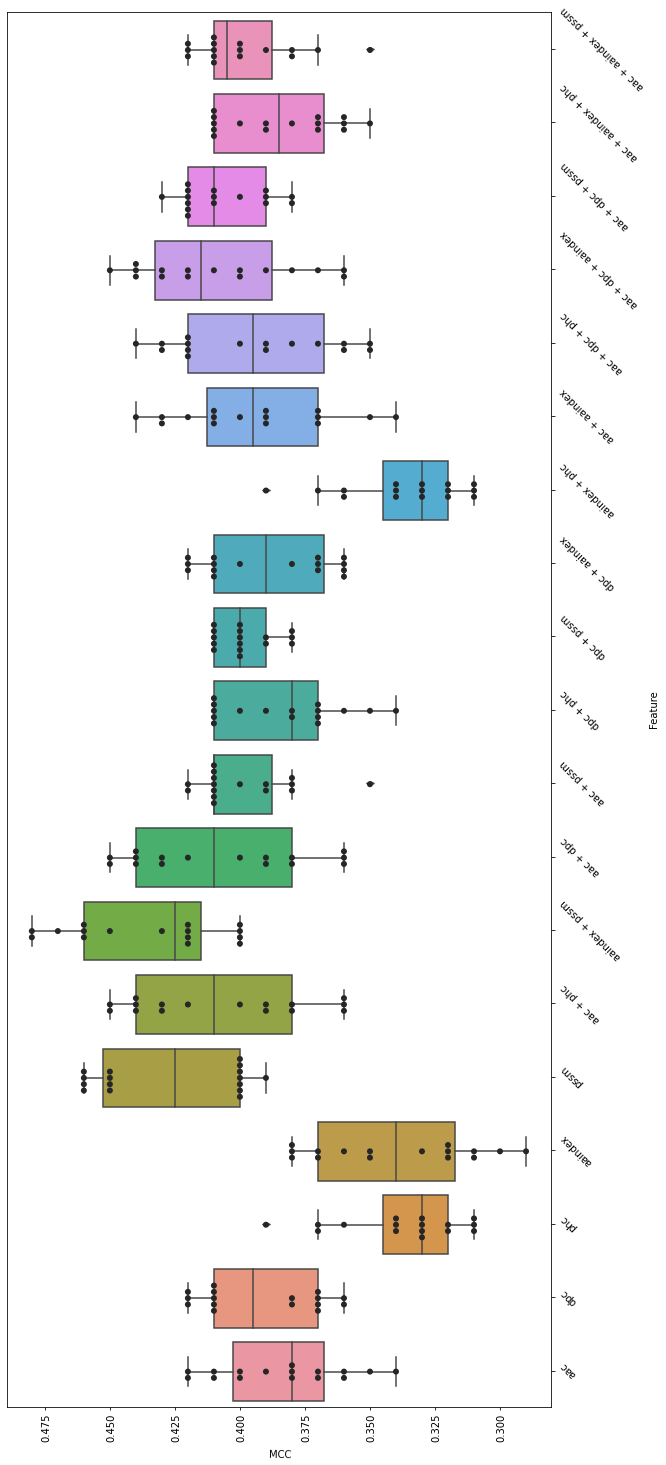
\includegraphics[width=14cm,height=21cm]{figures/15MccAllModels.png}
    \caption{MCC results from applying the closest 10\% models to all the features.
    The hybrid model that included the AAindex and the PSSM profile (7th box), outperforms others.}
    \label{fig:MccAllModels}
\end{figure}
